\section{Group Solar Collectors}\label{group-solar-collectors}

Solar collectors are thermal devices that convert solar energy into thermal energy by raising the temperature of a circulating heat transfer fluid. The fluid can then be used to heat water for domestic hot water usage or space heating.

In EnergyPlus solar collectors are components that are connected to the plant loop. A solar heating system can be constructed with a combination of solar collectors, pumps, and hot water tanks.

Flate plate solar collectors are defined using two objects: \hyperref[solarcollectorflatplatewater]{SolarCollector:FlatPlate:Water} and \hyperref[solarcollectorperformanceflatplate]{SolarCollectorPerformance:FlatPlate}. Similarly, Integral-Collector-Storage (ICS) solar collectors are defined using two objects: \hyperref[solarcollectorintegralcollectorstorage]{SolarCollector:IntegralCollectorStorage}, and \hyperref[solarcollectorperformanceintegralcollectorstorage]{SolarCollectorPerformance:IntegralCollectorStorage}. The \hyperref[solarcollectorflatplatewater]{SolarCollector:FlatPlate:Water} and \hyperref[solarcollectorintegralcollectorstorage]{SolarCollector:IntegralCollectorStorage} objects describe the plant component connections. These object also reference \hyperref[solarcollectorperformanceflatplate]{SolarCollectorPerformance:FlatPlate} and \hyperref[solarcollectorperformanceintegralcollectorstorage]{SolarCollectorPerformance:IntegralCollectorStorage} performance objects which contains the thermal and optical performance test data for a specific make and model of collector. Parameters are defined separately so that these values can be organized into a reference data set and need only be entered once if for an array of the same type of collectors.

\subsection{SolarCollector:FlatPlate:Water}\label{solarcollectorflatplatewater}

The flat-plate solar collector model simulates glazed, unglazed, and tubular (i.e.~evacuated tube) collectors. The SolarCollector:FlatPlate:Water object represents a single collector module connected to the plant loop. The thermal and optical properties of the collector module are taken from the referenced \hyperref[solarcollectorperformanceflatplate]{SolarCollectorPerformance:FlatPlate} object. A surface or shading object defines the collector tilt, azimuth, and gross area. The collector surface participates normally in all shading calculations if the ``FullExterior,'' ``FullInteriorAndExterior,'' FullExteriorWithReflections , or FullInteriorAndExteriorWithReflections flags are set in the Solar Distribution field of the Building object. Inlet and outlet nodes are specified for plant connections on the demand side of the plant loop.

\subsubsection{Inputs}\label{inputs-045}

\paragraph{Field: Name}\label{field-name-044}

The unique name of the SolarCollector:FlatPlate:Water object.

\paragraph{Field: Solar Collector Performance Name}\label{field-solar-collector-performance-name}

Reference name of a \hyperref[solarcollectorperformanceflatplate]{SolarCollectorPerformance:FlatPlate} object that defines the thermal and optical properties of the collector.

\paragraph{Field: Surface Name}\label{field-surface-name-005}

Reference to one of the many different types of surfaces such as the \hyperref[buildingsurfacedetailed]{BuildingSurface:Detailed} or the \hyperref[shadingzonedetailed-000]{Shading:Zone:Detailed} objects. The surface named here is used to define the solar collector tilt, azimuth, and gross area.

\paragraph{Field: Inlet Node Name}\label{field-inlet-node-name-007}

The name of the inlet node connection to the plant loop.

\paragraph{Field: Outlet Node Name}\label{field-outlet-node-name-008}

The name of the outlet node connection to the plant loop.

\paragraph{Field: Maximum Flow Rate}\label{field-maximum-flow-rate-002}

The maximum flow rate {[}m\(^{3}\)/s{]} allowed through the collector. This field is optional. If not specified, the collector will allow as much flow as the rest of the plant can deliver.

An example follows.

\begin{lstlisting}

SolarCollector:FlatPlate:Water,
  Collector 1,                                                       !- Name
  ACR Solar International Fireball 2001,   !- Solar Collector Performance Name
  Collector Surface,                                           !- Surface Name
  Collector Inlet Node,                                     !- Inlet Node Name
  Collector Outlet Node,                                   !- Outlet Node Name
  0.00005;                                                               !- Maximum Flow Rate (m3/s)
\end{lstlisting}

\subsubsection{Outputs}\label{outputs-034}

The following output variables are reported for the SolarCollector:FlatPlate:Water object:

\begin{itemize}
\item
  HVAC,Average,Solar Collector Incident Angle Modifier {[]}
\item
  HVAC,Average,Solar Collector Efficiency {[]}
\item
  HVAC,Average,Solar Collector Heat Transfer Rate {[}W{]}
\item
  HVAC,Average,Solar Collector Heat Gain Rate {[}W{]}
\item
  HVAC,Average,Solar Collector Heat Loss Rate {[}W{]}
\item
  HVAC,Sum,Solar Collector Heat Transfer Energy {[}J{]}
\end{itemize}

\paragraph{Solar Collector Incident Angle Modifier {[]}}\label{solar-collector-incident-angle-modifier}

The incident angle modifier is an important intermediate value used in the SRCC calculation of solar collector performance. The value reported here is the combined result for the current time that includes incident angles of beam solar, diffuse solar from sky, and diffuse solar from ground.

\paragraph{Solar Collector Efficiency {[]}}\label{solar-collector-efficiency}

The overall collector efficiency. This is the ratio of collected energy and the incident solar energy. The efficiency can be greater than 1 at times when the outdoor air temperature is warm enough.

\paragraph{Solar Collector Heat Transfer Rate {[}W{]}}\label{solar-collector-heat-transfer-rate-w}

\paragraph{Solar Collector Heat Transfer Energy {[}J{]}}\label{solar-collector-heat-transfer-energy-j}

These are the overall rate (in W) and amount of energy ( in J) transferred to the collector's circulating fluid. Positive values indicate heating of the fluid while negative values indicate cooling of the fluid.

\paragraph{Solar Collector Heat Gain Rate {[}W{]}}\label{solar-collector-heat-gain-rate-w}

This is the overall rate of heat addition to the collector's circulating fluid in Watts. Values are always positive or zero. If the fluid is actually cooled then the value is zero.

\paragraph{Solar Collector Heat Loss Rate {[}W{]}}\label{solar-collector-heat-loss-rate-w}

This is the overall rate of heat loss from the collector's circulating fluid in Watts. Values are always positive or zero. If the fluid is actually heated then the value is zero.

In addition, several surface variables are also relevant for the collector's surface object (BuildingSurface:Detailed or Shading:Zone:Detailed):

\begin{itemize}
\item
  Zone,Average,Surface Outside Face Sunlit Area {[}m2{]}
\item
  Zone,Average,Surface Outside Face Sunlit Fraction {[]}
\item
  Zone,Average,Surface Outside Face Incident Solar Radiation Rate per Area {[}W/m2{]}
\item
  Zone,Average,Surface Outside Face Incident Beam Solar Radiation Rate per Area {[}W/m2{]}
\item
  Zone,Average,Surface Outside Face Incident Sky Diffuse Solar Radiation Rate per Area {[}W/m2{]}
\item
  Zone,Average,Surface Outside Face Incident Ground Diffuse Solar Radiation Rate per Area {[}W/m2{]}
\item
  Zone,Average,Surface Outside Face Beam Solar Incident Angle Cosine Value {[]}
\end{itemize}

The temperatures at the inlet and outlet nodes and the collector mass flow rate can be monitored using the system node output variables:

\begin{itemize}
\item
  HVAC,Average,System Node Temperature {[}C{]}
\item
  HVAC,Average,System Node Mass Flow Rate {[}kg/s{]}
\end{itemize}

\subsection{SolarCollectorPerformance:FlatPlate}\label{solarcollectorperformanceflatplate}

The SolarCollectorPerformance:FlatPlate object contains the thermal and optical performance parameters for a single collector module. These parameters are based on the testing methodologies described in ASHRAE Standards 93 and 96. The Solar Rating and Certification Corporation (SRCC) applies these standards in their rating procedures of solar collectors. The ratings for commercially available collectors in North America are published in the \emph{Directory of SRCC Certified Solar Collector Ratings}. The SRCC database has also been converted into an EnergyPlus data set of SolarCollectorPerformance:FlatPlate objects that is included with the program (see SolarCollectors.idf in the DataSets folder).

The coefficients for the energy conversion efficiency and incident angle modifier allow first order (linear) or second order (quadratic) correlations. To use a first order correlation, the second order coefficient must be left blank or set to zero.

In order for the model to work correctly, the test conditions for which the performance coefficients were measured must be specified in the fields: \emph{Test Fluid}, \emph{Test Volumetric Flow Rate}, and \emph{Test Correlation Type}. Currently, only water is allowed as the \emph{Test Fluid}.

For more detailed information about the performance coefficients, see the \emph{EnergyPlus Engineering Reference Document}.

\subsubsection{Inputs}\label{inputs-1-042}

\paragraph{Field: Name}\label{field-name-1-041}

The unique name of the SolarCollectorPerformance:FlatPlate object.

\paragraph{Field: Gross Area}\label{field-gross-area}

The gross area of the collector module {[}m\(^{2}\){]}. This value is mainly for reference. The area of the associated collector surface object is used in all calculations.

\paragraph{Field: Test Fluid}\label{field-test-fluid}

The fluid that was used in the testing procedure that resulted in the thermal and optical performance coefficients below. Currently only Water is allowed. This the fluid during the collector testing, not the fluid used during a particular EnergyPlus run.

\paragraph{Field: Test Flow Rate}\label{field-test-flow-rate}

The volumetric flow rate during testing {[}m\(^{3}\)/s{]}. If the value is available as flow rate per unit area, it is recommended to multiply by the \emph{Gross Area} of the collector module, not the net aperture area.

\paragraph{Field: Test Correlation Type}\label{field-test-correlation-type}

This field specifies type of temperature used to develop the correlation equations. The testing procedure is based on an experimental correlation using either Inlet, Average, or Outlet temperature. Enter one of these choices. The ASHRAE Standards 93 and 96 always use Inlet temperature.

\paragraph{Field: Coefficient 1 of Efficiency Equation}\label{field-coefficient-1-of-efficiency-equation}

First coefficient of efficiency equation for energy conversion {[}dimensionless{]}. This is the Y-intercept term.

\paragraph{Field: Coefficient 2 of Efficiency Equation}\label{field-coefficient-2-of-efficiency-equation}

Second coefficient of efficiency equation for energy conversion {[}W/m\(^{2}\)-K{]}. This is the first-order term.

\paragraph{Field: Coefficient 3 of Efficiency Equation}\label{field-coefficient-3-of-efficiency-equation}

Third coefficient of efficiency equation for energy conversion {[}W/m\(^{2}\)-K\(^{2}\){]}. This field is optional. This is the second-order term. If left blank or set to zero, a first-order linear correlation is used.

\paragraph{Field: Coefficient 2 of Incident Angle Modifier}\label{field-coefficient-2-of-incident-angle-modifier}

Second coefficient of the incident angle modifier equation. This the first-order term. (There is no \emph{Coefficient 1 of Incident Angle Modifier} because that number is always 1.0.)

\paragraph{Field: Coefficient 3 of Incident Angle Modifier}\label{field-coefficient-3-of-incident-angle-modifier}

Third coefficient of the incident angle modifier equation. This is the second-order term. This field is optional. If left blank or set to zero, a first order linear correlation is used.

An example of this object follows.

\begin{lstlisting}

SolarCollectorPerformance:FlatPlate,
  Alternate Energy Technologies AE-32,   !- Name
  2.9646,                                   !- Gross Area {m2}
  WATER,                                     !- Test Fluid
  0.0000388,                             !- Test Flow Rate {m3/s}
  INLET,                                     !- Test Correlation Type
  0.691,                                     !- Coefficient 1 of Efficiency Equation {dimensionless}
  -3.396,                                   !- Coefficient 2 of Efficiency Equation {W/m2-K}
  -0.00193,                               !- Coefficient 3 of Efficiency Equation {W/m2-K2}
  -0.1939,                                 !- Coefficient 2 of Incident Angle Modifier
  -0.0055;                                 !- Coefficient 3 of Incident Angle Modifier
\end{lstlisting}

\subsubsection{Outputs}\label{outputs-1-025}

This object does not generate any output; see SolarCollector:FlatPlate:Water Output

\subsection{SolarCollector:IntegralCollectorStorage}\label{solarcollectorintegralcollectorstorage}

The Integral-Collector-Storage (ICS) solar collector model simulates glazed collectors with integral storage unit. The SolarCollector:IntegralCollectorStorage object represents a single collector module connected to the plant loop. The thermal and optical properties of the collector module are calculated from inputs in \hyperref[solarcollectorperformanceintegralcollectorstorage]{SolarCollectorPerformance:IntegralCollectorStorage} object. A surface or shading object defines the collector tilt, and azimuth. The collector surface participates normally in all shading calculations if the ``FullExterior,'' ``FullInteriorAndExterior,'' FullExteriorWithReflections , or FullInteriorAndExteriorWithReflections flags are set in the Solar Distribution field of the Building object. Inlet and outlet nodes are specified for plant connections on the demand side of the plant loop. The \hyperref[surfacepropertyexteriornaturalventedcavity]{SurfaceProperty:ExteriorNaturalVentedCavity}, object is required to describe the surface properties, the characteristics of the cavity and opening for natural ventilation if OtherSideConditionsModel is specified as the collector bottom surface outside boundary condition type.

\subsubsection{Inputs}\label{inputs-2-039}

\paragraph{Field: Name}\label{field-name-2-036}

The unique name of the SolarCollector:IntegralCollectorStorage object.

\paragraph{Field: Solar Collector Performance Name}\label{field-solar-collector-performance-name-1}

Reference name of a \hyperref[solarcollectorperformanceintegralcollectorstorage]{SolarCollectorPerformance:IntegralCollectorStorage} object that defines the thermal and optical properties of the collector.

\paragraph{Field: Surface Name}\label{field-surface-name-1-001}

Reference to one of the many different types of surfaces such as the \hyperref[buildingsurfacedetailed]{BuildingSurface:Detailed} or the \hyperref[shadingzonedetailed-000]{Shading:Zone:Detailed} objects. The surface named here is used to define the solar collector tilt, and azimuth. The collector shades the surface it is mounted on and hence impacts the surface heat balance.

\paragraph{Field: Bottom surface Boundary Conditions Type}\label{field-bottom-surface-boundary-conditions-type}

This field contains the type of boundary conditions applicable to the ICS collector bottom surface. Allowed boundary condition types are: AmbientAir and OtherSideConditionsModel. If the other side conditions model is selected, specify the name of the \hyperref[surfacepropertyothersideconditionsmodel]{SurfaceProperty:OtherSideConditionsModel} object in the next input field, otherwise, leave the next input field blank. The AmbientAir boundary condition uses outdoor air temperature as boundary condition, hence the subsurface is assumed to be exposed to the sun and wind.

\paragraph{Field: Other Side Conditions Model Name}\label{field-other-side-conditions-model-name}

This field contains the name of a \hyperref[surfacepropertyothersideconditionsmodel]{SurfaceProperty:OtherSideConditionsModel} object declared elsewhere in the input file. This will connect the collector to the exterior boundary conditions for the underlying heat transfer surface specified above..

\paragraph{Field: Inlet Node Name}\label{field-inlet-node-name-1-004}

The name of the inlet node connection to the plant loop.

\paragraph{Field: Outlet Node Name}\label{field-outlet-node-name-1-005}

The name of the outlet node connection to the plant loop.

\paragraph{Field: Maximum Flow Rate}\label{field-maximum-flow-rate-1-000}

The maximum flow rate {[}m3/s{]} allowed through the collector. This field is optional. If not specified, the collector will allow as much flow as the rest of the plant can deliver.

An example follows.

\begin{lstlisting}

SolarCollector:IntegralCollectorStorage,
  Collector 1,                                                       !- Name
  ICS Solar Collector,                                       !- Solar Collector Performance Name
  ICS Collector Surface,                                   !- Surface Name
  OtherSideConditionsModel,                             !- Bottom Surface Boundary Conditions Type
  ICS OSCM,                                                             !- Boundary Condition Model Name
  Collector Inlet Node,                                     !- Inlet Node Name
  Collector Outlet Node,                                   !- Outlet Node Name
  0.00005;                                                               !- Maximum Flow Rate (m3/s)
\end{lstlisting}

\subsection{SolarCollectorPerformance:IntegralCollectorStorage}\label{solarcollectorperformanceintegralcollectorstorage}

The SolarCollectorPerformance:IntegralCollectorStorage object contains the thermal and optical performance parameters for a single collector module. The transmittance-absorptance product of the absorber and cover system is determined from optical properties specified. For more detailed information about the calculation procedure, see the \emph{EnergyPlus Engineering Reference} Document.

\subsubsection{Inputs}\label{inputs-3-035}

\paragraph{Field: Name}\label{field-name-3-030}

The unique name of the SolarCollectorPerformance:IntegralCollectorStorage object.

\paragraph{Field: ICS Collector Type}\label{field-ics-collector-type}

This input field is the ICS collector type. Currently only RectangularTank type is allowed.

\paragraph{Field: Gross Area}\label{field-gross-area-1}

This input field is the gross area of the collector module in m2. This gross area is used in the energy balance equations.

\paragraph{Field: Collector Water Volume}\label{field-collector-water-volume}

This input field is the volume of water in the solar collector in m3.

\paragraph{Field: Bottom Heat Loss Conductance}\label{field-bottom-heat-loss-conductance}

This input field is the collector bottom heat loss conductance in W/m2K. This value is calculated from thermal conductivity and thickness of the bottom insulation.

\paragraph{Field: Side Heat Loss Conductance}\label{field-side-heat-loss-conductance}

This input field is the collector side heat loss conductance in W/m2K. This value is calculated from thermal conductivity and thickness of the side insulation.

\paragraph{Field: Collector Aspect Ratio}\label{field-collector-aspect-ratio}

This input field is the ratio of the short side (width) of the collector to the long side (length) of the collector. This value is used only for calculating the collector side area along with the collector side height specified in the next input filed. This ratio is less or equal to 1.0.

\paragraph{Field: Collector Side Height}\label{field-collector-side-height}

This input field is height of collector side in m. This height is used to estimate the collector side area for heat loss calculations along with heat loss coefficient specified in the input field above.

\paragraph{Field: Thermal Mass of Absorber Plate}\label{field-thermal-mass-of-absorber-plate}

This input field is thermal-mass of the absorber plate per unit area of the collector in {[}J/m2×K{]}. This input value multiplied by the absorber gross area determines the thermal mass of the absorber plate. It is estimated from the specific heat, density and average thickness of the absorber plate. If zero is specified then the absorber plate energy balance reduces to steady state form.

\paragraph{Field: Number of Covers}\label{field-number-of-covers}

Number of transparent collector covers. Common practice is to use two covers: glass as the outer cover and Teflon as the inner cover. If single cover is specified leave the inner cover optical and thermal properties input fields blank.

\paragraph{Field: Cover Spacing}\label{field-cover-spacing}

This input field provides the spacing between the two transparent covers, and the spacing between the inner cover and the absorber plate in m. Default value is 0.05m.

\paragraph{Field: Refractive Index of Outer Cover}\label{field-refractive-index-of-outer-cover}

This is the average Refractive index for solar spectrum range of the outer transparent cover material. Glass is used as the outer cover. Average refractive index value for non-absorbing glass used in solar collectors over solar spectrum range is 1.526.

\paragraph{Field: Extinction Coefficient Times Thickness of Outer Cover}\label{field-extinction-coefficient-times-thickness-of-outer-cover}

This input field is the product of the extinction coefficient and the thickness of the out cover material. The extinction coefficient for glass types approximately varies from 4m\(^{-1}\) to 32 m\(^{-1}\). The extinction coefficient for low-iron glass, which is the default outer cover material, is 15 m\(^{-1}\). The default value for extinction coefficient times thickness (KL) is 0.045 ( = 15.0 x0.003), which is the product of the default extinction coefficient of 15m\(^{-1}\) and 3.0mm thick glass.

\paragraph{Field: Emissivity of Outer Cover}\label{field-emissivity-of-outer-cover}

This input field value is thermal emissivity of the outer collector cover. The default value assumes low-iron glass with thermal emissivity of 0.88.

\paragraph{Field: Refractive Index of Inner Cover}\label{field-refractive-index-of-inner-cover}

This input field is the average Refractive index of the inner transparent cover of the collector. Commonly Teflon (PolytetraFluoroethylene) is used as the inner cover. The average refractive index value over the solar spectrum range for Teflon is 1.37.

\paragraph{Field: Extinction Coefficient Times Thickness of Inner Cover}\label{field-extinction-coefficient-times-thickness-of-inner-cover}

This input field is the product of the extinction coefficient (K) and the thickness (L) of the inner cover material. The inner cover material is more transparent than the out cover, very thin and hence their thickness can be assumed to be negligible. The default value for extinction coefficient times thickness (KL) is 0.008 ( = 40.0x0.0002), which is the product of extinction coefficient of 40m\(^{-1}\) and a thickness of 0.2mm.

\paragraph{Field: Emissivity of Inner Cover}\label{field-emissivity-of-inner-cover}

This input field value is thermal emissivity of the inner transparent collector cover. The default value assumes plastic sheet with thermal emissivity of 0.30. This value is used in the thermal analysis only.

\paragraph{Field: Absorptance of Absorber Plate}\label{field-absorptance-of-absorber-plate}

This input field is shortwave or solar absorptance of the absorber plate. The default value is 0.96.

\paragraph{Field: Emissivity of Absorber Plate}\label{field-emissivity-of-absorber-plate}

This input field value is thermal emissivity of the absorber plate. Default value is 0.30. This input value is used in the thermal analysis only.

An example follows.

\begin{lstlisting}

SolarCollectorPerformance:IntegralCollectorStorage,
  ICS Experimental,               !- Name
  RectangularTank,                 !- ICS Collector Type
  0.37275,                                 !- Gross Area {m2}
  0.0195875,                             !- Collector Water Volume {m3}
  0.10,                                       !- Bottom Heat Loss Conductance
  1.00,                                       !- Side Heat Loss Conductance
  0.8,                                         !- Collector Aspect Ratio {dimensionless}
  0.08,                                       !- Collector Side Height {m}
  5800.0,                                         !- Thermal Mass of Absorber Plate {J/m2K}
  1,                                             !- Number of Covers {dimensionless}
  0.05,                                       !- Cover Spacing {m}
  1.526,                                     !- Refractive Index of Outer Cover {dimensionless}
  0.0125,           !- Extinction Coefficient Times Thickness of Outer Cover {dimensionless}
  0.88,                                       !- Emissivity of Outer Cover
  1.126,                                     !- Refractive Index of Inner Cover {dimensionless}
  0.0126,           !- Extinction Coefficient Times Thickness of Inner Cover {dimensionless}
  0.88,                                       !- Emissivity of Inner Cover {dimensionless}
  0.96,                                       !- Absorptance of Absorber Plate {dimensionless}
  0.60;                                       !- Emissivity of Absorber Plate {dimensionless}
\end{lstlisting}

\subsubsection{Outputs}\label{outputs-2-020}

The following output variables are reported for the SolarCollector:IntegralCollectorStorage object:

\begin{itemize}
\item
  HVAC,Average,Solar Collector Storage Water Temperature {[}C{]}
\item
  HVAC,Average,Solar Collector Absorber Plate Temperature {[}C{]}
\item
  HVAC,Average,Solar Collector Overall Top Heat Loss Coefficient {[}W/m2-C{]}
\item
  HVAC,Average,Solar Collector Thermal Efficiency {[]}
\item
  HVAC,Average,Solar Collector Storage Heat Transfer Rate {[}W{]}
\item
  HVAC,Sum,Solar Collector Storage Heat Transfer Energy {[}J{]}
\item
  HVAC,Average,Solar Collector Heat Transfer Rate {[}W{]}
\item
  HVAC,Sum,Solar Collector Heat Transfer Energy {[}J{]}
\item
  HVAC,Average,Solar Collector Skin Heat Transfer Rate {[}W{]}
\item
  HVAC,Sum, Solar Collector Skin Heat Transfer Energy {[}J{]}
\item
  HVAC,Average,Solar Collector Transmittance Absorptance Product {[]}
\end{itemize}

\paragraph{Solar Collector Storage Water Temperature {[}C{]}}\label{solar-collector-storage-water-temperature-c}

This output variable is the ICS collector stored water average temperature at a given time steps in degree Celsius. This temperature is the same as the collector ICS collector leaving water temperature.

\paragraph{Solar Collector Absorber Plate Temperature {[}C{]}}\label{solar-collector-absorber-plate-temperature-c}

This output variable is the ICS collector absorber plate average temperature at a given time steps in degree Celsius.

\paragraph{Solar Collector Thermal Efficiency {[]}}\label{solar-collector-thermal-efficiency}

This output variable is the instantaneous thermal efficiency of the ICS solar collector in per cent. This value is determined from net useful energy collected and the total incident solar radiation for each time step. The net useful energy collected is the sum of the energy stored in the collector and net useful energy delivered.

\paragraph{Solar Collector Storage Heat Transfer Rate {[}W{]}}\label{solar-collector-storage-heat-transfer-rate-w}

\paragraph{Solar Collector Storage Heat Transfer Energy {[}J{]}}\label{solar-collector-storage-heat-transfer-energy-j}

These output variables are the instantaneous rate of change of the energy and the change in energy of the water in the ICS solar collector in Watts, and Joules, respectively.

\paragraph{Solar Collector Skin Heat Transfer Rate {[}W{]}}\label{solar-collector-skin-heat-transfer-rate-w}

\paragraph{Solar Collector Skin Heat Transfer Energy {[}J{]}}\label{solar-collector-skin-heat-transfer-energy-j}

These output variables are the instantaneous skin heat loss rate and the heat loss energy of the ICS solar collector for each time steps in Watts, and Joules respectively. The skin heat loss rate is the sum of the heat losses through the top, bottom and sides of the collector surfaces. This value is mostly negative, but can have a positive value (heat gain) when the outdoor air temperature is warmer than the collector.

\paragraph{Solar Collector Heat Transfer Rate {[}W{]}}\label{solar-collector-heat-transfer-rate-w-1}

\paragraph{Solar Collector Heat Transfer Energy {[}J{]}}\label{solar-collector-heat-transfer-energy-j-1}

This output variable is the heat rate and Energy transferred from the ICS collector to the collector loop fluid (water) in Watts and Joule, respectively. This value is determined from the collector water mass flow rate, specific heat of water and the temperature difference between the collector water outlet and inlet nodes at each time step. The value is positive when the fluid is heated or negative when cooled.

\paragraph{Solar Collector Transmittance Absorptance Product {[]}}\label{solar-collector-transmittance-absorptance-product}

This output variable is the transmittance-absorptance product of the covers and absorber system of the ICS solar collector. This value ranges from 0.0 to less than 1.0.

\paragraph{Solar Collector Overall Top Heat Loss Coefficient {[}W/m2-C{]}}\label{solar-collector-overall-top-heat-loss-coefficient-wm2-c}

This output variable is the overall heat loss coefficient from the absorber plate to the ambient air calculated for each time step.

\subsection{SolarCollector:FlatPlate:PhotovoltaicThermal}\label{solarcollectorflatplatephotovoltaicthermal}

This object is used to model hybrid photovoltaic-thermal (PVT) solar collectors that convert incident solar energy into both electricity and useful thermal energy. This object describes the PVT solar collector by referencing other objects that provide more detail or connections to other parts of the EnergyPlus model.

The PVT solar collectors need to be connected to either an HVAC air system or a plant loop for collected thermal energy to be utilized. The input field for the type of thermal working fluid informs the program how the PVT collector is expected to be connected. If the the working fluid is air, then the PVT collectors are modeled as a ventilation air pretreatment component and connected to an outdoor air system. If the working fluid is water, then the PVT collectors are modeled as a hot water solar collector and are connected to a plant loop with a water thermal storage tank.

\subsubsection{Inputs}\label{inputs-4-032}

\paragraph{Field: Name}\label{field-name-4-027}

This field should contain a unique name chosen by the user to identify a specific PVT collector in the building model.

\paragraph{Field: Surface Name}\label{field-surface-name-2-001}

This field is the user-defined name of a surface object (defined elsewhere) to which the PVT module is attached. These can be any type of building surface that is exposed to the exterior environment. The model uses the named surface's geometry for the PVT solar collector.

\paragraph{Field: Photovoltaic-Thermal Model Performance Name}\label{field-photovoltaic-thermal-model-performance-name}

This field is the user-defined name of an object (defined elsewhere) that provides the performance details of the PVT module. This should be the name of a \hyperref[solarcollectorperformancephotovoltaicthermalsimple]{SolarCollectorPerformance:PhotovoltaicThermal:Simple} object. Multiple different SolarCollector:FlatPlate:PhotovoltaicThermal objects can reference the same object that provides performance details.

\paragraph{Field: Photovoltaic Generator Name}\label{field-photovoltaic-generator-name}

This field is the user-defined name of a \hyperref[generatorphotovoltaic-000]{Generator:Photovoltaic} object (defined elsewhere) that will be used to model the solar electric portion of the PVT solar collector. The PVT models make any adjustments needed to model PV performance in the context of the PVT collector.

\paragraph{Field: Thermal Working Fluid Type}\label{field-thermal-working-fluid-type}

This field is the user's choice for the type of fluid used to collect thermal energy. PVT solar collectors can capture thermal energy in either air or water streams. The choices available for this field are Water or Air. If the choice is Air then the PVT collector needs to be connected to an HVAC air system loop. The PVT collector should be situated as the first component on an outdoor air inlet stream. If the choice is Water then the PVT collector needs to be connected to a Plant water system loop. The connections are made via node names which are defined in the following fields, depending on the working fluid type.

\paragraph{Field: Water Inlet Node Name}\label{field-water-inlet-node-name-003}

This field is the name of Plant loop node that serves as the inlet to the PVT collector. This field is only used if the Thermal Working Fluid Type is set to Plant/Water.

\paragraph{Field: Water Outlet Node Name}\label{field-water-outlet-node-name-002}

This field is the name of a plant loop node that seves as the outlet from the PVT collector. This field is only used if the Thermal Working Fluid Type is set to Plant/Water.

\paragraph{Field: Air Inlet Node Name}\label{field-air-inlet-node-name-006}

This field is the name of HVAC air loop node that serves as the inlet to the PVT collector. This field is only used if the Thermal Working Fluid Type is set to HVAC/Air.

\paragraph{Field: Air Outlet Node Name}\label{field-air-outlet-node-name-005}

This field is the name of HVAC air loop node that serves as the outlet from the PVT collector. This field is only used if the Thermal Working Fluid Type is set to HVAC/Air.

\paragraph{Field: Design Flow Rate}\label{field-design-flow-rate-003}

This field is used to describe the nominal volume flow rate of the thermal working fluid. The units are m3/s. The volume flow rate is autosizable.

An example of this object follows.

\begin{lstlisting}

SolarCollector:FlatPlate:PhotovoltaicThermal,
  PVT: 1_Ceiling ,                                             !- Name
  1_Ceiling ,                                                       !- Surface Name
  30percentPVThalfArea ,                                 !- Photovoltaic-Thermal Model Performance Name
  PV:ZN_1_FLR_1_SEC_1_Ceiling ,                   !- Photovoltaic Name
  Air ,                                                                   !- Thermal Working Fluid Type
  ,                                                                           !- Water Inlet Node Name
  ,                                                                           !- Water Outlet Node Name
  ZN_1_FLR_1_SEC_1:Sys_OAInlet Node ,       !- Air Inlet Node Name
  PVT:ZN_1_FLR_1_SEC_1_Ceiling Outlet ,   !- Air Outlet Node Name
  Autosize ;                                                         !- Design Flow Rate
\end{lstlisting}

\subsubsection{Outputs}\label{outputs-3-018}

The output variables that are available for flat plate PVT include the following.

\begin{itemize}
\item
  HVAC,Average,Generator Produced Thermal Rate {[}W{]}
\item
  HVAC,Sum,Generator Produced Thermal Energy {[}J{]}
\item
  HVAC,Average,Generator PVT Fluid Bypass Status {[]}
\item
  HVAC,Average,Generator PVT Fluid Inlet Temperature {[}C{]}
\item
  HVAC,Average,Generator PVT Fluid Outlet Temperature {[}C{]}
\item
  HVAC,Average,Generator PVT Fluid Mass Flow Rate {[}kg/s{]}
\end{itemize}

\paragraph{Generator Produced Thermal Rate {[}W{]}}\label{generator-produced-thermal-rate-w-000}

\paragraph{Generator Produced Thermal Energy {[}J{]}}\label{generator-produced-thermal-energy-j-000}

These outputs are the thermal energy and power produced by the PVT collector. PVT collectors are a type of cogenerator, producing both electrical and thermal power and these variables report the thermal portion in the same manner as other fuel-based cogenerators. The thermal energy is placed on HeatProduced meter and is attributed to SolarWater or SolarAir depending on the type of working fluid. The generator thermal production is also reported at the load center level.

\paragraph{Generator PVT Fluid Bypass Status {[]}}\label{generator-pvt-fluid-bypass-status}

This output variable indicates the status a bypass damper. It is only available for air-based PVT. There are no dimensions and the range is between 0.0 and 1.0. If the value is 0.0, then there is no bypassing and all the working fluid goes through the collector. If the value is 1.0, then there is complete bypassing and all the working fluid goes around the collector. If the value is between 0.0 and 1.0, then the model is effectively mixing bypass and collector streams to target a temperature setpoint placed on the outlet node.

\paragraph{Generator PVT Fluid Inlet Temperature {[}C{]}}\label{generator-pvt-fluid-inlet-temperature-c}

This report is the inlet temperature of the working fluid that enters the PVT collector

\paragraph{Generator PVT Fluid Outlet Temperature {[}C{]}}\label{generator-pvt-fluid-outlet-temperature-c}

This report is the outlet temperature of the working fluid that leaves the PVT collector

\paragraph{Generator PVT Fluid Mass Flow Rate {[}kg/s{]}}\label{generator-pvt-fluid-mass-flow-rate-kgs}

This report is the mass flow rate of the working fluid through the PVT collector. This is the overall mass flow rate, portions of the flow may be internally bypassed around the collector itself for control modulation.

\subsection{SolarCollectorPerformance:PhotovoltaicThermal:Simple}\label{solarcollectorperformancephotovoltaicthermalsimple}

This object is used to provide performance details for the simple PVT model. This is a simple user-defined efficiency model. Thermal conversion efficiency is a constant or scheduled value. There are no output variable for this object, reporting is done by the parent PVT object.

\subsubsection{Inputs}\label{inputs-5-029}

\paragraph{Field: Name}\label{field-name-5-023}

This field is the unique name for this object.

\paragraph{Field: Fraction of Surface Area with Active Thermal Collector}\label{field-fraction-of-surface-area-with-active-thermal-collector}

This field is the fraction of the surface area that is active. It should be a decimal fraction between 0.0 and 1.0. The area of the PVT s surface will be multiplied by this fraction to determine the active area of the PVT collector(s).

\paragraph{Field: Thermal Conversion Efficiency Input Mode Type}\label{field-thermal-conversion-efficiency-input-mode-type}

This field is used to determine how the thermal efficiency is input. There are two choices, Fixed or Scheduled. If this field is set to Fixed, then a constant value for thermal efficiency will be used (set in next field). If this field is set to Scheduled, then the thermal efficiency values are defined in a schedule.

\paragraph{Field: Value for Thermal Conversion Efficiency if Fixed}\label{field-value-for-thermal-conversion-efficiency-if-fixed}

This field is used to provide a value for the efficiency with which solar energy is collected in the working fluid. This field is only used if the input mode is set to Fixed in the previous field. Efficiency is defined as the thermal energy collected divided by the incident solar radiation. The value should be between 0.0 and 1.0. The user should be careful that the thermal efficiency and the electrical efficiency be consistent with each other because the overall efficiency of the PVT collector is the combination of both thermal and electrical.

\paragraph{Field: Name of Schedule for Thermal Conversion Efficiency}\label{field-name-of-schedule-for-thermal-conversion-efficiency}

This field is used for the name of a schedule that provides values for the efficiency with which solar energy is collected in the working fluid. This field is only used if the input mode is set to Scheduled in the field above. Efficiency is defined as the thermal energy collected divided by the incident solar radiation. The values in the named schedule should be between 0.0 and 1.0. The user should be careful that the thermal efficiency and the electrical efficiency be consistent with each other because the overall efficiency of the PVT collector is the combination of both thermal and electrical.

\paragraph{Field: Front Surface Emittance}\label{field-front-surface-emittance}

This field is used to describe an average value for the total hemispherical emittance of the collector's front face exposed to the sky. This is used to model cooling applications where the PVT collectors are operated at night to cool the working fluid.

An example input object follows.

\begin{lstlisting}

SolarCollectorPerformance:PhotovoltaicThermal:Simple,
  20percentEffPVhalfArea ,                 !- Name
  0.5 ,                                                       !- Fraction of Surface Area with Active Thermal Collector
  Fixed ,                                                   !- Thermal Conversion Efficiency Input Mode Type
  0.2 ,                                                       !- Value for Thermal Conversion Efficiency if Fixed
  ,                                                             !- Name of Schedule for Thermal Conversion Efficiency
  0.84 ;                                                     !- Front Surface Emittance
\end{lstlisting}

\subsection{Solar Collector Heating System Plant Connections}\label{solar-collector-heating-system-plant-connections}

This section provides an overview of how to model solar heating systems. A solar heating system can be constructed using a combination of solar collectors, pumps, water tanks and water heaters. The solar collector must be connected on the demand side of the plant loop. Multiple collector modules can be combined in series and parallel using the normal plant connection rules. The supply side of the plant loop should contain a water heater with the solar collector loop connecting to the \emph{Source Side Inlet} and \emph{Source Side Outlet} nodes. As usual, the pump must be the first component on the supply side.

If the solar heating system is for domestic hot water (or service water heating) usage only, the field \emph{Use Flow Rate Fraction Schedule Name} of the \hyperref[waterheatermixed]{WaterHeater:Mixed} object can be used to avoid additional plant connections. If the system has more complicated hot water requirements or if the system is for space heating, the \emph{Use Side Inlet} and \emph{Use Side Outlet} nodes must be connected to another plant loop to serve zone and non-zone equipment. (See the \hyperref[waterheatermixed]{WaterHeater:Mixed} object documentation for more information.)

\begin{figure}[hbtp] % fig 132
\centering
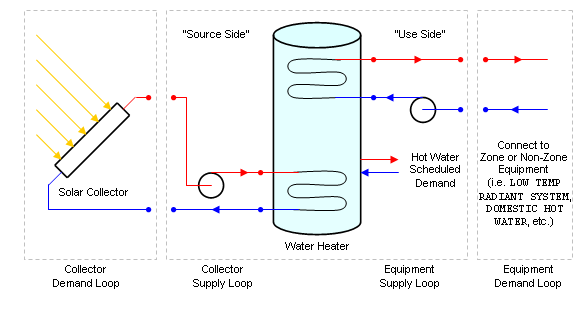
\includegraphics[width=0.9\textwidth, height=0.9\textheight, keepaspectratio=true]{media/image339.png}
\caption{Solar Collector Plant Loop Connection Diagram \protect \label{fig:solar-collector-plant-loop-connection-diagram}}
\end{figure}

NOTE: The EnergyPlus plant simulation requires the pump to be the first component on the supply side. This may be different from the way the solar heating system is actually configured. This should not affect the validity of the simulation results.

In order to realize energy savings with a solar heating system, it is best to use a two-tank system with a storage tank and auxiliary water heater. The storage tank gathers heat directly from the solar collectors and stores it for later use. The storage tank is modeled using a \hyperref[waterheatermixed]{WaterHeater:Mixed} object with the \emph{Heater Maximum Capacity} set to zero. The auxiliary water heater is positioned downstream of the storage tank on the supply side of the main plant loop. The auxiliary water heater, or booster water heater, provides additional heat if the storage tank water is not hot enough. The auxiliary water heater can be modeled as an instantaneous/tankless water heater or as a standard tanked water heater with heating source (see \hyperref[waterheatermixed]{WaterHeater:Mixed}).

\begin{figure}[hbtp] % fig 133
\centering
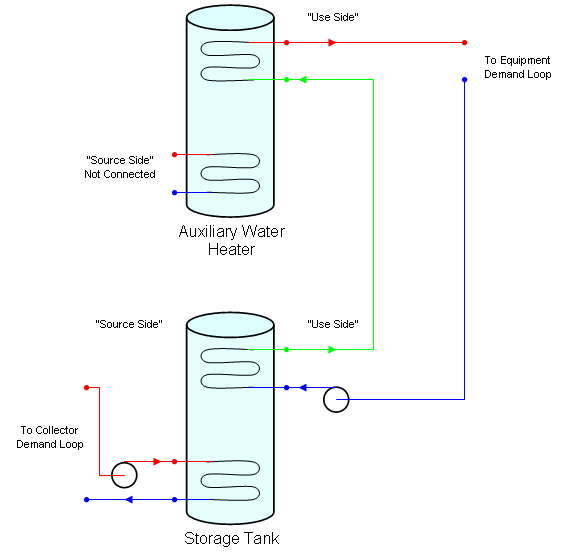
\includegraphics[width=0.9\textwidth, height=0.9\textheight, keepaspectratio=true]{media/image340.png}
\caption{Two-Tank Solar Heating System Connection Diagram \protect \label{fig:two-tank-solar-heating-system-connection}}
\end{figure}

Another strategy to consider for solar heating systems is to allow the storage tank to reach a much higher temperature than necessary for the end use. This allows the tank to store more energy from the solar collectors, when it is available. However, for applications such as domestic hot water, it is undesirable and unsafe to supply excessive hot water temperatures at the point of demand. To take advantage of higher storage temperatures, yet still avoid scalding temperatures at the faucet, the hot water leaving the storage tank can be tempered with cold water using a three-way valve to achieve the target temperature. See the \hyperref[temperingvalve]{TemperingValve} object documentation for more details.

A complete two-tank solar heating system with tempering valve is shown below.

\begin{figure}[hbtp] % fig 134
\centering
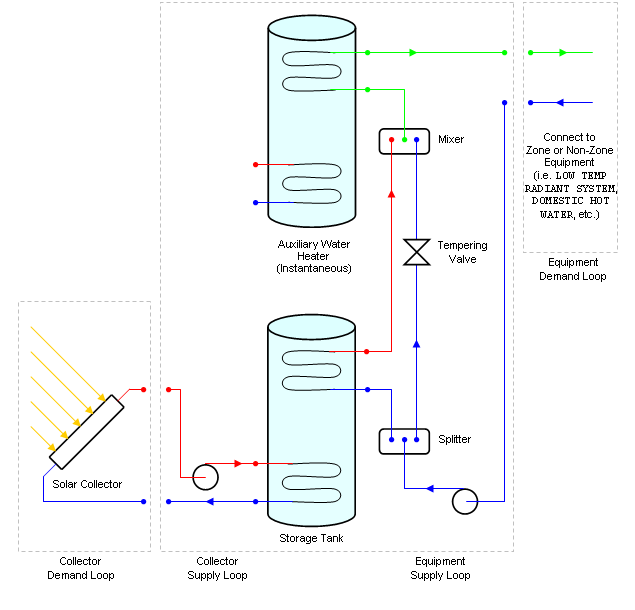
\includegraphics[width=0.9\textwidth, height=0.9\textheight, keepaspectratio=true]{media/image341.png}
\caption{Two-Tank Solar Heating System with Tempering Valve \protect \label{fig:two-tank-solar-heating-system-with-tempering}}
\end{figure}

\subsection{Solar Heating System Control}\label{solar-heating-system-control}

There are several options for controlling a solar heating system in EnergyPlus. Since the solar collectors request a constant flow demand based on their \emph{Maximum Flow Rate}, the limiting factor is actually the flow rate determined by the loop pump. Therefore the entire system can be controlled using the \emph{Pump Flow Rate Schedule} of the pump. If the schedule is omitted, the pump and system will run all the time (without any other controls specified). This is usually not the best way to operate a solar heating system.

To better control the collector loop, a differential thermostat can be used to compare the temperature in the water heater to the temperature in the collector so that the pump is only turned on when there is a useful heat gain. The differential thermostat is simulated using the \hyperref[availabilitymanagerdifferentialthermostat]{AvailabilityManager:DifferentialThermostat} object. For a typical system, the \emph{Hot Node Name} field refers to an outlet node of one of the collector modules. The \emph{Cold Node Name} field refers to the \emph{Source Side Outlet} node, i.e.~the cold storage water leaving the water heater. The fields \emph{Temperature Difference On Limit} and \emph{Temperature Difference Off Limit} are usually 8 12 C and 1 3 C respectively. If the two temperature differences are too close, it is possible for the system to turn on and off rapidly without much useful heat gain. This can also occur if the flow rate through the collector is too high. Without flow the fluid in the collector heats up more quickly; when high flow is turned on, all of the hot fluid is removed and the temperature drops, forcing the system off again.

Another control method is to use a photovoltaic panel to power the pump. The system begins pumping when there is enough solar radiation to operate the pump. This is not yet implemented in EnergyPlus.

\subsubsection{Freeze Prevention}\label{freeze-prevention}

In climates with a cold season, the solar heating system must be designed to avoid the risk of fluid freezing in the solar collector or exposed pipes and causing damage. This is not a problem if air is the heat transfer fluid. With water, however, there are several strategies that can minimize the risk.

\emph{Seasonal schedule}. The simplest strategy is to not use the system during the cold season. This is a hassle because it requires the collector to be manually drained of all fluid. The benefits of the solar heating system are also lost during this time. This can be simulated in EnergyPlus with the appropriate pump schedule for the collector system.

\emph{Antifreeze}. The freezing point of the liquid is decreased by adding antifreeze to the water or using a different heat transfer liquid with a lower freezing point. This cannot yet be simulated in EnergyPlus because only pure water is currently allowed in plant loops.

\emph{Drain-back system}. This strategy automatically empties the collector when the pump is not running. This scenario is modeled by default in EnergyPlus, although the extra pump energy required to start the system is not taken into account.

\emph{Recirculation system}. This strategy automatically recirculates warm liquid from the storage tank back through the collector to maintain the system above the freezing point. There are system losses using this method. This can be simulated in EnergyPlus by using \hyperref[availabilitymanagerlowtemperatureturnon]{AvailabilityManager:LowTemperatureTurnOn} to force the system to turn on when the outdoor air temperature or collector outlet temperature falls below a specified minimum.

\subsubsection{Additional Controls}\label{additional-controls}

In addition to freeze prevention, it is also necessary to prevent the system from becoming too hot. This is usually a safety issue for the water heater. For this case it is important to have a high temperature cutoff to stop the pump before damaging the water heater. This is accomplished with a \hyperref[availabilitymanagerhightemperatureturnoff]{AvailabilityManager:HighTemperatureTurnOff}.

\subsubsection{System Availability Manager List Example}\label{system-availability-manager-list-example}

To use the availability managers for the control cases described above, a \hyperref[availabilitymanagerassignmentlist]{AvailabilityManagerAssignmentList} must be defined and referenced in the \hyperref[plantloop]{PlantLoop} object of the collector loop. An example of a differential thermostat, recirculation for freeze prevention, and high temperature cutoff is shown below:

\begin{lstlisting}

AvailabilityManagerAssignmentList,
  Collector Loop Availability Manager List,             !- Name
  AvailabilityManager:HighTemperatureTurnOff,         !- Availability Manager 1 Object Type
  High Temperature Turn Off Availability Manager, !- Availability Manager 1 Name
  AvailabilityManager:HighTemperatureTurnOn,           !- Availability Manager 2 Object Type
  Low Temperature Turn On Availability Manager,     !- Availability Manager 2 Name
  AvailabilityManager:DifferentialThermostat,         !- Availability Manager 3 Object Type
  Differential Thermostat Availability Manager;     !- Availability Manager 3 Name


  AvailabilityManager:HighTemperatureTurnOff,           ! For water heater safety
  High Temperature Turn Off Availability Manager, !- Name
  Water Heater Use Outlet Node,                                     !- Sensor Node Name
  60.0;                                                                                     !- Temperature (C)


  AvailabilityManager:HighTemperatureTurnOn,             ! For freeze prevention by recirculation
  Low Temperature Turn On Availability Manager,     !- Name
  Collector Outlet Node,                                                   !- Sensor Node Name
  0.0;                                                                                       !- Temperature (C)


  AvailabilityManager:DifferentialThermostat,           ! For useful heat gain from collector to tank
  Differential Thermostat Availability Manager,     !- Name
  Collector Outlet Node,                                                   !- Hot Node Name
  Water Heater Source Outlet Node,                               !- Cold Node Name
  .0,                                                                                     !- Temperature Difference On Limit (delta C)
  2.0;                                                                                       !- Temperature Difference Off Limit (delta C)
\end{lstlisting}

The \hyperref[availabilitymanagerdifferentialthermostat]{AvailabilityManager:DifferentialThermostat} object must always be the last manager in the availability manager list. See the \hyperref[availabilitymanagerassignmentlist]{AvailabilityManagerAssignmentList} object documentation for more information.

\subsection{SolarCollector:UnglazedTranspired}\label{solarcollectorunglazedtranspired}

This object is used to model unglazed transpired solar collectors (UTSC) used to condition outdoor air. These collectors are generally used to heat air drawn through perforated absorbers that are heated by the sun and also recover heat conducted out through the underlying wall. The SolarCollector:UnglazedTranspired object represents a single collector attached to one or more \hyperref[buildingsurfacedetailed]{BuildingSurface:Detailed} objects and to one or more outdoor air systems. Therefore the transpired collector is part of both the thermal envelope and the HVAC system. An example file is provided called TranspiredCollectors.idf.

The area and orientation of the collector is obtained from \hyperref[buildingsurfacedetailed]{BuildingSurface:Detailed} objects, which are referenced by name. Although the collector surface itself is slightly detached from the underlying building wall (or roof), no additional surface object is needed to represent the collector itself. When modeling transpired collectors, it is important to consider the size of the collector when developing the building model's \hyperref[buildingsurfacedetailed]{BuildingSurface:Detailed} objects because the underlying surfaces must match the collector. For example, if the collector covers only part of the wall, then that wall should be split into separate surfaces where one matches the size of the collector. A single collector can be associated with as many \hyperref[buildingsurfacedetailed]{BuildingSurface:Detailed} objects as desired since this object is extensible. The collector can be arranged at any tilt angle by describing the surfaces appropriately. The surfaces need not be contiguous nor have the same orientation, but the program will issue warnings if surfaces have widely ranging tilts and azimuths.

The collector conditions outdoor air and is connected to the outdoor air system using the usual method of specifying node names. Using the UTSC model requires specifying a relatively complete HVAC air system that includes an outdoor air path. This will typically require using a set of objects that, at a minimum, will include: \hyperref[airloophvaccontrollerlist]{AirLoopHVAC:ControllerList}, \hyperref[airloophvacoutdoorairsystemequipmentlist]{AirLoopHVAC:OutdoorAirSystem:EquipmentList}, \hyperref[airloophvacoutdoorairsystem]{AirLoopHVAC:OutdoorAirSystem}, \hyperref[outdoorairnodelist]{OutdoorAir:NodeList}, \hyperref[outdoorairmixer]{OutdoorAir:Mixer}, \hyperref[setpointmanagermixedair]{SetpointManager:MixedAir}, and \hyperref[controlleroutdoorair]{Controller:OutdoorAir}. A single UTSC can serve more than one outdoor air system but requires also using a separate object, called \hyperref[solarcollectorunglazedtranspiredmultisystem]{SolarCollector:UnglazedTranspired:Multisystem} to specify node connections.

Controls for the UTSC involve setting the rate of air flow and the status of a bypass damper. If the bypass damper is open, then all the ventilation air goes straight into the outdoor air mixer; if it closed, then all the air first passes through the UTSC. The bypass damper is modeled as completely open or completely closed. The UTSC bypass damper control is determined by an availability manager, the airflow set by the outdoor air mixer controls, and thermostatic type controls that decide if heating is useful. An availability schedule is used to bypass the collector for certain times of the year, eg. summer cooling season. The air flow rates are set by controls associated with the outdoor air mixer (see \hyperref[setpointmanagermixedair]{SetpointManager:MixedAir}, and \hyperref[controlleroutdoorair]{Controller:OutdoorAir}). Thermostatic type control decides if the collector will provide useful heating based on either of two types of setpoints. The first type of temperature setpoint is managed by \hyperref[setpointmanagermixedair]{SetpointManager:MixedAir}, where the UTSC model looks at a control node, usually the mixed air node. The second type is an extra setpoint especially for free heating that is managed within this object where the UTSC model looks at the zone air node.

\subsubsection{Inputs}\label{inputs-6-026}

\paragraph{Field: Name}\label{field-name-6-021}

This field contains a unique name for the unglazed transpired solar collector.

\paragraph{Field: Boundary Conditions Model Name}\label{field-boundary-conditions-model-name-000}

This field contains the name of a \hyperref[surfacepropertyothersideconditionsmodel]{SurfaceProperty:OtherSideConditionsModel} object declared elsewhere in the input file. This will connect the collector to the exterior boundary conditions for the underlying heat transfer surface.

\paragraph{Field: Availability Schedule Name}\label{field-availability-schedule-name-016}

This field contains the name of a schedule that determines whether or not the UTSC is available. When the schedule value is less than or equal to zero, the UTSC is always bypassed. When the schedule value is greater than zero, the UTSC is available and will be used when other conditions are met, such as outdoor air requested by mixer and preheating has been determined to be beneficial based on thermostatic control. If this field is blank, the schedule has values of 1 for all time periods.

\paragraph{Field: Inlet Node Name}\label{field-inlet-node-name-2-003}

This field contains the name of an air node that provides air into the UTSC. This node name should also be assigned to be an outdoor air node using the \hyperref[outdoorairnodelist]{OutdoorAir:NodeList} or \hyperref[outdoorairnode]{OutdoorAir:Node} objects. This node should also be named as the actuated node in a \hyperref[controlleroutdoorair]{Controller:OutdoorAir} object. If the UTSC is connected to more than one air system, then this field can be left blank and the \hyperref[solarcollectorunglazedtranspiredmultisystem]{SolarCollector:UnglazedTranspired:Multisystem} object should be used to define the nodes.

\paragraph{Field: Outlet Node Name}\label{field-outlet-node-name-2-003}

This field contains the name of an air node that is the outlet of the UTSC. This node name will typically be the inlet to the \hyperref[outdoorairmixer]{OutdoorAir:Mixer} (if there is no other equipment on the outdoor air path). If the UTSC is connected to more than one air system, then this field can be left blank and the \hyperref[solarcollectorunglazedtranspiredmultisystem]{SolarCollector:UnglazedTranspired:Multisystem} object should be used to define the nodes.

\paragraph{Field: Setpoint Node Name}\label{field-setpoint-node-name-000}

This field contains the name of an air node that has a setpoint manager controlling its temperature setpoint. This node name will typically be named as the control node in a a \hyperref[controlleroutdoorair]{Controller:OutdoorAir} object. If the UTSC is connected to more than one air system, then this field can be left blank and the \hyperref[solarcollectorunglazedtranspiredmultisystem]{SolarCollector:UnglazedTranspired:Multisystem} object should be used to define the nodes.

\paragraph{Field: Zone Node Name}\label{field-zone-node-name-001}

This field contains the name of an air node for a thermal zone that is ultimately connected to the air system. This node is used with the setpoint schedule, defined in the following field, to provide an added layer of thermostatic control for the UTSC without affecting the control of auxiliary heating. If there is a single air system that is connected to more than one zone, then a single zone should be selected based on where the thermostat might be located. If the UTSC is connected to more than one air system, then this field can be left blank and the \hyperref[solarcollectorunglazedtranspiredmultisystem]{SolarCollector:UnglazedTranspired:Multisystem} object should be used to define the nodes.

\paragraph{Field: Free Heating Setpoint Schedule Name}\label{field-free-heating-setpoint-schedule-name}

This field contains the name of a temperature schedule defined elsewhere in the input file. This schedule should define temperatures \emph{desired} in the zone, but not necessarily \emph{required}. This secondary setpoint schedule is used to allow the UTSC to operate as if it has its own thermostat that is separate from the primary control mechanism. When the UTSC is used with auxiliary heating, the usual setpoint managers and temperature controllers will determine how the auxiliary heaters are controlled. This allows using a higher zone air temperature setpoint for controlling UTSC bypass than for the auxiliary heating system.

\paragraph{Field: Diameter of Perforations in Collector}\label{field-diameter-of-perforations-in-collector}

This field is used to enter the effective diameter of the perforations in the collector surface. The diameter should be entered in meters. For perforations other than round, use an equivalent diameter for a round hole that would have the same area.

\paragraph{Field: Distance Between Perforations in Collector}\label{field-distance-between-perforations-in-collector}

This field is used to enter the pitch, or average, shortest distance between perforations.

\paragraph{Field: Thermal Emissivity of Collector Surface}\label{field-thermal-emissivity-of-collector-surface}

This field is used to enter the thermal emissivity of the collector. This surface property is for longwave infrared radiation. The property is used for both sides of collector. Most painted materials have an emissivity of 0.9.

\paragraph{Field: Solar Absorbtivity of Collector Surface}\label{field-solar-absorbtivity-of-collector-surface}

This field is used to enter the solar absorbtivity of the collector. This surface property is for shortwave, solar radiation. The property is used for the front side of the collector that faces the environment. Darker colors have a higher absorbtivity. While black is the highest performance, other colors might be used to match the color scheme of the rest of the facade. The following table provides sample solar absorbtivities for different colors (source: Conserval Engineering Inc., Toronto, Ontario, Canada).

\begin{longtable}[c]{@{}ll@{}}
\toprule
Color Name of Kynar(R) [[1]](\#\_ftn1) Paint & Solar Absorptivity \tabularnewline
\midrule
\endfirsthead

\toprule
Color Name of Kynar(R) [[1]](\#\_ftn1) Paint & Solar Absorptivity \tabularnewline
\midrule
\endhead

Black & 0.94 \tabularnewline
Classic Bronze & 0.91 \tabularnewline
Chocolate Brown & 0.9 \tabularnewline
Hartford Green & 0.9 \tabularnewline
Med. Bronze & 0.89 \tabularnewline
Boysenberry & 0.86 \tabularnewline
Rocky Grey & 0.85 \tabularnewline
Regal Blue & 0.85 \tabularnewline
Forest Green & 0.84 \tabularnewline
Hemlock Green & 0.82 \tabularnewline
Slate Blue & 0.8 \tabularnewline
Redwood & 0.79 \tabularnewline
Teal & 0.79 \tabularnewline
Slate Grey & 0.79 \tabularnewline
Patina Green & 0.77 \tabularnewline
Mint Green & 0.71 \tabularnewline
Dove Grey & 0.69 \tabularnewline
Mission Red & 0.69 \tabularnewline
Sierra Tan & 0.65 \tabularnewline
Brite Red & 0.59 \tabularnewline
Rawhide & 0.57 \tabularnewline
Sandstone & 0.54 \tabularnewline
Silversmith & 0.53 \tabularnewline
Coppertone & 0.51 \tabularnewline
Concord Cream & 0.45 \tabularnewline
Ascot White & 0.4 \tabularnewline
Bone White & 0.3 \tabularnewline
\bottomrule
\end{longtable}

(\protect\hyperlink{ux5fftnref1}{{[}1{]}} Kynar is a registered trademark of Elf Atochem North America, Inc.)

\paragraph{Field: Effective Overall Height of Collector}\label{field-effective-overall-height-of-collector}

This field is used to enter a nominal height for the collector. This value is used in the program to determine a length scale in the vertical direction for the buoyancy-driven portion of natural ventilation that occurs when the collector is inactive. (Note that most of the geometry information is obtained from the underlying surfaces.) The value entered here is adjusted inside the program to account for tilt of the collector. While the value here would generally correspond to the actual distance/height, its value is not critical and it can be used to adjust modeling the air exchange rates in passive mode. If the collector is horizontal, then the length scale is obtained from the following field.

\paragraph{Field: Effective Gap Thickness of Plenum Behind Collector}\label{field-effective-gap-thickness-of-plenum-behind-collector}

This field is used to enter a nominal gap thickness for the collector. This distance value is only used when the collector is near horizontal to determine a length scale in the vertical direction for buoyancy calculations. For example, if the collector is mounted on a flat roof, its tilt-adjusted height is zero and the program will use this gap thickness as a length scale rather than the height from the previous field.

\paragraph{Field: Effective Cross Section Area of Plenum Behind Collector}\label{field-effective-cross-section-area-of-plenum-behind-collector}

This field is used to enter the nominal cross sectional area of the gap behind the collector. This area is used to determine a velocity scale for surface convection heat transfer correlations when the collector is active. This value is generally the average gap thickness times the average width of the collector.

\paragraph{Field: Hole Layout Pattern for Pitch}\label{field-hole-layout-pattern-for-pitch}

This field is used to describe the pattern of perforations in the collector surface. There are currently two choices available: Square and Triangle. Note that the hole layout pattern should be consistent with how the value for pitch was determined.

\paragraph{Field: Heat Exchange Effectiveness Correlation}\label{field-heat-exchange-effectiveness-correlation}

This field is used to select which correlation is used to model heat transfer from the collector surface to the incoming air when the collector is active. There are two choices available: Kutscher1994, and VanDeckerHollandsBrunger2001. See the Engineering Reference for details and references.

\paragraph{Field: Ratio of Actual Collector Surface Area to Projected Surface Area}\label{field-ratio-of-actual-collector-surface-area-to-projected-surface-area}

This field is used to enter a factor that accounts for the extra surface area resulting from corrugations in the collector surface. Corrugations help stiffen the collector. The projected surface area is obtained by the program from the (flat) underlying surfaces. If the collector is flat then this ratio is 1.0. If the collector is corrugated, then this ratio will be greater than one. A typical value might be 1.165.

\paragraph{Field: Roughness of Collector}\label{field-roughness-of-collector}

This field is used to describe the relative roughness of the collector material. This field is similar to one in the \hyperref[material]{Material} object. This parameter only influences the convection coefficients, more specifically the outside convection coefficient. A special keyword is expected in this field with the options being VeryRough , Rough , MediumRough , MediumSmooth , Smooth , and VerySmooth in order of roughest to smoothest options.

\paragraph{Field: Collector Thickness}\label{field-collector-thickness}

This field is used to enter the thickness of the collector material. This value is only needed for the Van Decker Hollands Brunger 2001 correlation. The material thickness should be entered in meters.

\paragraph{Field: Effectiveness for Perforations with Respect to Wind}\label{field-effectiveness-for-perforations-with-respect-to-wind-000}

This field is used to enter a value for the coefficient used to determine natural air exchanges from wind, or Cv. When the collector is inactive, wind will cause exterior air to move in and out of the collector. Cv is an arbitrary coefficient used to model the effectiveness of openings and depends on opening geometry and the orientation with respect to the wind. Cv should probably be in the range 0.25 to 0.65. Increasing Cv will increase the amount of natural ventilation.

\paragraph{Field: Discharge Coefficient for Openings with Respect to Buoyancy Driven Flow}\label{field-discharge-coefficient-for-openings-with-respect-to-buoyancy-driven-flow-000}

This field is used to enter a value for the coefficient used to determine natural air exchanges from buoyancy, or Cd. When the collector is inactive, stack or buoyancy effects will cause exterior air to move in and out of the collector. Cd is an arbitrary discharge coefficient that depends on the geometry of the opening. Cd should probably be in the range 0.4 to 1.0. Increasing Cd will increase the amount of natural ventilation.

\paragraph{Field: Surface \textless{}\#\textgreater{} Name}\label{field-surface-name-3-001}

The remaining fields are used to name the \hyperref[buildingsurfacedetailed]{BuildingSurface:Detailed} objects that are associated with the UTSC. These are the underlying heat transfer surfaces and are defined elsewhere in the input file. These other surfaces should all specify OtherSideConditionsModel as their exterior environment. This object is extensible, so additional fields of this type can be added to the end of this object.

An example of this object follows.

\begin{lstlisting}

SolarCollector:UnglazedTranspired,
  Shop OA UTSC ZN11,                               ! Name
  UTSC OSCM ZN11,                                     ! Boundary Conditions Model Name
  HeatingAvailSched ,                             ! Availability Schedule Name
  Outside Air Inlet Node ZN11 ,         ! Inlet Node Name
  UTSC Outlet Node ZN11 ,                     ! Outlet Node Name
  Mixed Air Node ZN11 ,                         ! Setpoint Node Name
  ZN11 Node,                                               ! Zone Node Name
  ShopFreeHeatingSetpoints,                 ! Free Heating Setpoint Schedule Name
  0.0016,                                                     ! Diameter of Perforations in Collector
  0.01689,                                                   ! Distance Between Perforations in Collector
  0.9,                                                           ! Thermal Emissivity of Collector Surface
  0.9,                                                           ! Solar Absorbtivity of Collector Surface
  4.0,                                                           ! Effective Overall Height of Collector
  0.1,                                                           ! Effective Gap Thickness of Plenum Behind Collector
  2.0,                                                           ! Effective Cross Section Area of Plenum Behind Collector
  Triangle,                                                 ! Hole Layout Pattern for Pitch
  Kutscher1994,                                         ! Heat Exchange Effectiveness Correlation
  1.165,                                           ! Ratio of Actual Collector Surface Area to Projected Surface Area
  MediumRough ,                                         ! Roughness of Collector
  0.00086,                                                   ! Collector Thickness
  0.25,                                                         ! Effectiveness for Perforations with Respect to Wind
  0.5,                                 ! Discharge Coefficient for Openings with Respect to Buoyancy Driven Flow
  ZN11_Shop_1:ExtWall:South;               ! Surface 1 Name
\end{lstlisting}

\subsubsection{Outputs}\label{outputs-4-015}

In addition to related output that can be obtained for air nodes and surfaces, these outputs are available for UTSC systems:

\begin{itemize}
\item
  HVAC,Average,Solar Collector Heat Exchanger Effectiveness {[]}
\item
  HVAC,Average,Solar Collector Leaving Air Temperature {[}C{]}
\item
  HVAC,Average,Solar Collector Outside Face Suction Velocity {[}m/s{]}
\item
  HVAC,Average,Solar Collector Surface Temperature {[}C{]}
\item
  HVAC,Average,Solar Collector Plenum Air Temperature {[}C{]}
\item
  HVAC,Average,Solar Collector Sensible Heating Rate {[}W{]}
\item
  Zone,Meter,SolarAir:Facility {[}J{]}
\item
  Zone,Meter,SolarAir:HVAC {[}J{]}
\item
  Zone,Meter,HeatProduced:SolarAir {[}J{]}
\item
  HVAC,Sum,Solar Collector Sensible Heating Energy {[}J{]}
\item
  HVAC,Average,Solar Collector Natural Ventilation Air Change Rate {[}ACH{]}
\item
  HVAC,Average,Solar Collector Natural Ventilation Mass Flow Rate {[}kg/s{]}
\item
  HVAC,Average,Solar Collector Wind Natural Ventilation Mass Flow Rate {[}kg/s{]}
\item
  HVAC,Average,Solar Collector Buoyancy Natural Ventilation Mass Flow Rate {[}kg/s{]}
\item
  HVAC,Average,Solar Collector Incident Solar Radiation {[}W/m2{]}
\item
  HVAC,Average,Solar Collector System Efficiency {[]}
\item
  HVAC,Average,Solar Collector Surface Efficiency {[]}
\end{itemize}

\paragraph{Solar Collector Heat Exchanger Effectiveness {[]}}\label{solar-collector-heat-exchanger-effectiveness}

The results from UTSC correlations defined by \({\varepsilon_{HX}} = \frac{{{T_{a,HX}} - {T_{amb}}}}{{{T_{s,coll}} - {T_{amb}}}}\) .

\paragraph{Solar Collector Leaving Air Temperature {[}C{]}}\label{solar-collector-leaving-air-temperature-c}

The temperature of air entering the plenum after being heated by the collector. When there is no forced air flow or the collector is passive, then the condition of air entering the plenum or the collector leaving air is assumed to be that of outside air.

\paragraph{Solar Collector Outside Face Suction Velocity {[}m/s{]}}\label{solar-collector-outside-face-suction-velocity-ms}

The bulk velocity of air approaching the collector.

\paragraph{Solar Collector Surface Temperature {[}C{]}}\label{solar-collector-surface-temperature-c}

The surface temperature of the collector itself.

\paragraph{Solar Collector Plenum Air Temperature {[}C{]}}\label{solar-collector-plenum-air-temperature-c}

The temperature of air inside, and leaving, the plenum behind the collector. This plenum leaving air temperature depends on the mode of operation of the collector. When the collector is passive (no forced flow), then the passive model assumes the condition of air entering the plenum is that of outside air, or else when the collector is active, then the model sets the plenum entering air condition to transpired collector leaving air condition determined from the collector model.

\paragraph{Solar Collector Sensible Heating Rate {[}W{]}}\label{solar-collector-sensible-heating-rate-w}

The overall rate at which heat is being added to the outdoor air stream.

\paragraph{SolarAir:Facility {[}J{]}}\label{solarairfacility-j}

A meter that includes the heating energy provided by the UTSC.

\paragraph{SolarAir:HVAC {[}J{]}}\label{solarairhvac-j}

A meter that includes the heating energy provided by the UTSC.

\paragraph{HeatProduced:SolarAir {[}J{]}}\label{heatproducedsolarair-j}

A meter that includes the heating energy provided by the UTSC.

\paragraph{Solar Collector Sensible Heating Energy {[}J{]}}\label{solar-collector-sensible-heating-energy-j}

The overall sum of energy added to the outdoor air stream.

\paragraph{Solar Collector Natural Ventilation Air Change Rate {[}ACH{]}}\label{solar-collector-natural-ventilation-air-change-rate-ach}

The rate of natural ventilation air exchange between the plenum and ambient when the collector is inactive in Air Changes per Hour.

\paragraph{Solar Collector Natural Ventilation Mass Flow Rate {[}kg/s{]}}\label{solar-collector-natural-ventilation-mass-flow-rate-kgs}

The mass flow rate of natural ventilation air exchange between the plenum and ambient when the collector is inactive.

\paragraph{Solar Collector Wind Natural Ventilation Mass Flow Rate {[}kg/s{]}}\label{solar-collector-wind-natural-ventilation-mass-flow-rate-kgs}

The part of mass flow rate of natural ventilation air exchange between the plenum and ambient when the collector is inactive due to wind-driven forces.

\paragraph{Solar Collector Buoyancy Natural Ventilation Mass Flow Rate {[}kg/s{]}}\label{solar-collector-buoyancy-natural-ventilation-mass-flow-rate-kgs}

The part of mass flow rate of natural ventilation air exchange between the plenum and ambient when the collector is inactive due to buoyancy-driven forces.

\paragraph{Solar Collector Incident Solar Radiation {[}W/m2{]}}\label{solar-collector-incident-solar-radiation-wm2}

The intensity of solar radiation incident on the UTSC collector from all sources.

\paragraph{Solar Collector System Efficiency {[]}}\label{solar-collector-system-efficiency}

The overall efficiency of the UTSC system including collected solar energy and heat recovered from the underlying surface.

\paragraph{Solar Collector Surface Efficiency {[]}}\label{solar-collector-surface-efficiency}

The efficiency of the UTSC solar collector.

\subsection{SolarCollector:UnglazedTranspired:Multisystem}\label{solarcollectorunglazedtranspiredmultisystem}

This object is used to model unglazed transpired solar collectors (UTSC) that are connected to multiple outdoor air systems. This object supplements the \hyperref[solarcollectorunglazedtranspired]{SolarCollector:UnglazedTranspired} object and is only necessary if more than one air system is connected to a single transpired collector. After the name field, there are sets of four node names used to define the connections of each air system. Each set contains node names for inlet, outlet, control, and zone.

\subsubsection{Field: Solar Collector Name}\label{field-solar-collector-name}

This field is used to identify the name of the \hyperref[solarcollectorunglazedtranspired]{SolarCollector:UnglazedTranspired} object that needs to be connected to more than one air system. This field must match the name.

\subsubsection{Field Set: Inlet Node, Outlet Node, Mixed Air Node, Zone Node}\label{field-set-inlet-node-outlet-node-mixed-air-node-zone-node}

This object is extensible, so the following four fields can be repeated as needed. One set is used for each outdoor air system that is connected to the collector.

\subsubsection{Field: Outdoor Air System \textless{}\#\textgreater{} Collector Inlet Node}\label{field-outdoor-air-system-collector-inlet-node}

This field contains the name of an air node that provides air into the UTSC. This node name should also be assigned to be an outdoor air node using the \hyperref[outdoorairnodelist]{OutdoorAir:NodeList} and \hyperref[outdoorairnode]{OutdoorAir:Node} objects. This node is also be named as the actuator node in a \hyperref[controlleroutdoorair]{Controller:OutdoorAir} object.

\subsubsection{Field: Outdoor Air System \textless{}\#\textgreater{} Collector Outlet Node}\label{field-outdoor-air-system-collector-outlet-node}

This field contains the name of an air node that is the outlet of the UTSC. This node name will typically be the Outdoor Air Stream Node Name in the \hyperref[outdoorairmixer]{OutdoorAir:Mixer} (if there is no other equipment on the outdoor air path).

\subsubsection{Field: Outdoor Air System \textless{}\#\textgreater{} Mixed Air Node}\label{field-outdoor-air-system-mixed-air-node}

This field contains the name of an air node that has a setpoint manager controlling its temperature setpoint. This node name will typically be named as the mixed air node in a \hyperref[controlleroutdoorair]{Controller:OutdoorAir} object.

\subsubsection{Field: Outdoor Air System \textless{}\#\textgreater{} Zone Node}\label{field-outdoor-air-system-zone-node}

This field contains the name of an air node for a thermal zone that is ultimately connected to the air system. This node is used with the setpoint schedule, defined in the following field, to provide an added layer of thermostatic control for the UTSC without affecting the control of auxiliary heating. If there is a single air system that is connected to more than one zone, then a single zone should be selected based on where the thermostat might be located.

An example of this object follows.

\begin{lstlisting}

SolarCollector:UnglazedTranspired:Multisystem,
  OFFICE MultiSystem OA UTSC ,   ! Solar Collector Name
  Outside Air Inlet Node ZN1,     ! Outdoor Air System 1 Collector Inlet Node
  UTSC Outlet Node ZN1,                 ! Outdoor Air System 1 Collector Outlet Node
  Mixed Air Node ZN1,                     ! Outdoor Air System 1 Mixed Air Node
  ZN1 Node,                                         ! Outdoor Air System 1 Zone Node
  Outside Air Inlet Node ZN2,     ! Outdoor Air System 2 Collector Inlet Node
  UTSC Outlet Node ZN2,                 ! Outdoor Air System 2 Collector Outlet Node
  Mixed Air Node ZN2,                     ! Outdoor Air System 2 Mixed Air Node
  ZN2 Node,                                         ! Outdoor Air System 2 Zone Node
  Outside Air Inlet Node ZN3,     ! Outdoor Air System 3 Collector Inlet Node
  UTSC Outlet Node ZN3,                 ! Outdoor Air System 3 Collector Outlet Node
  Mixed Air Node ZN3,                     ! Outdoor Air System 3 Mixed Air Node
  ZN3 Node,                                         ! Outdoor Air System 3 Zone Node
  Outside Air Inlet Node ZN4,     ! Outdoor Air System 4 Collector Inlet Node
  UTSC Outlet Node ZN4,                 ! Outdoor Air System 4 Collector Outlet Node
  Mixed Air Node ZN4,                     ! Outdoor Air System 4 Mixed Air Node
  ZN4 Node,                                         ! Outdoor Air System 4 Zone Node
  Outside Air Inlet Node ZN5,     ! Outdoor Air System 5 Collector Inlet Node
  UTSC Outlet Node ZN5,                 ! Outdoor Air System 5 Collector Outlet Node
  Mixed Air Node ZN5,                     ! Outdoor Air System 5 Mixed Air Node
  ZN5 Node;                                         ! Outdoor Air System 5 Zone Node
\end{lstlisting}